% =======================================================================
% UPDATED EXPERIMENTS SECTION — drop-in replacement for Section 4
% =======================================================================
% Changes from previous version:
%   - Updated v1 numbers to match new runs (passive_full=False, seed=1)
%   - Added full v3 (Qwen2.5 + BGE) subsection
%   - Replaced old .png figure references with new .pdf figures
%   - Fixed "Value-Gated" → "Confidence-Gated" (Problem 12)
%   - Added alpha-decay acknowledgment (Problem 4)
%   - Added CORRAL discussion (Problem 5)
%   - Added v3 results table
%   - Updated cross-dataset discussion
% =======================================================================

\section{Experiments}
\label{sec:experiments}

\subsection{General Experimental Setup}

\textbf{Datasets.} We evaluate the empirical performance of our Confidence-Gated meta-algorithm on two large-scale textual contextual bandit datasets characterized by massive action spaces, summarized in Table~\ref{tab:datasets}. We formulate the objective as a strict Precision@1 task: the algorithm receives a binary reward of $r_t = 1$ for selecting a correct ground-truth action, and $r_t = 0$ otherwise.

\begin{table}[h]
\centering
\caption{Summary of datasets used for contextual bandit experiments.}
\label{tab:datasets}
\begin{tabular}{@{}lcc@{}}
\toprule
\textbf{Dataset} & \textbf{Time Horizon ($T$)} & \textbf{Action Space ($|A|$)} \\ \midrule
OneShotWikiLinks-311 & 622,000 & 311 \\
AmazonCat-13K & 1,186,239 & 13,330 \\ \bottomrule
\end{tabular}
\end{table}

\textbf{Baselines \& Meta-Algorithm.} Each experiment simultaneously tracks three policies on the same data stream:
\begin{enumerate}[nosep]
    \item \textbf{Router (Algorithm~\ref{alg:confidence-gated}):} The confidence-gated meta-algorithm. We model the frozen LLM's design matrix as $V^{(1)} = c \cdot I_d$ with confidence parameter $c$, simplifying the LLM uncertainty score to $u_t^{(1)} = \|\phi(x_t, a_t^{(1)})\|_2 / \sqrt{c}$. The adaptive LinUCB's uncertainty is $u_t^{(0)} = \|\phi(x_t, a_t^{(0)})\|_{V_t^{-1}}$. The deterministic routing rule selects the LLM when $u_t^{(1)} < u_t^{(0)}$ and LinUCB otherwise.
    \item \textbf{LLM only (Pure Master):} A static frozen policy applied on every round, establishing the natural accuracy boundary.
    \item \textbf{Cold LinUCB (Pure Apprentice):} An independent LinUCB instance initialized from $\lambda I_d$ with no warm-start data.
\end{enumerate}

Regardless of which policy is selected by the Router, the adaptive learner's design matrix $V_t$ is updated with the played action's feature vector (covariance-only passive updates). The response vector $b_t$ is only updated on rounds where LinUCB is the active decision-maker. This matches the theoretical setting of Theorem~\ref{thm:warm-start-regret}, where passive covariance updates from the frozen policy precondition the design matrix without altering the reward signal.

\textbf{Exploration schedule.} We use a geometrically decaying exploration coefficient $\alpha_t = \max(0.1,\, 1.0 \cdot 0.9985^t)$, following standard empirical practice in neural-linear bandits. While the theoretical analysis assumes a fixed confidence radius $\beta_T$, the decaying schedule improves finite-horizon exploitation without affecting the qualitative predictions of the theory. In particular, the monotonic hand-off from frozen policy to LinUCB and the warm-start acceleration persist across different $\alpha$ schedules.

\textbf{Evaluation Metrics.} We measure learning efficiency using the Cumulative Average Reward (Precision@1). Mechanistically, we track the Fraction of LLM Routing over time to explicitly visualize the algorithm's ability to decay its reliance on the LLM.

% ==========================================
% WIKI RESULTS — v1 (Flan-T5 + BERT)
% ==========================================
\subsection{Flan-T5 Experiments on OneShotWikiLinks-311}
\label{sec:wiki_v1}

\paragraph{Environment Configuration.}
The OneShotWikiLinks-311 benchmark consists of 622{,}000 context--entity pairs spanning 311 entities (filtered for $\geq 2{,}000$ support). Context embeddings are produced by a frozen SentenceTransformer (\texttt{bert-base-nli-mean-tokens}), yielding $768$-dimensional vectors. Each entity is similarly embedded, producing a fixed action feature matrix $\Phi \in \mathbb{R}^{311 \times 768}$. The joint feature is the element-wise product $\phi(x,a) = x \odot a \in \mathbb{R}^{768}$. The frozen estimator is a Flan-T5 language model~\cite{chung2024scaling} used in mask-filling mode: the masked context is passed through T5, the predicted token is embedded, and the entity with highest cosine similarity to the prediction is selected. We experiment with three model sizes---\texttt{small} (60M parameters), \texttt{base} (250M), and \texttt{large} (780M)---which achieve progressively higher accuracy but are never updated online. The adaptive algorithm is LinUCB with Sherman--Morrison rank-1 updates, ridge regularization $\lambda = 0.1$, and batch size 128 (4{,}860 batches total). The confidence parameter is set uniformly to $c=100$ across all three LLM sizes; this eliminates $c$ as a confound and ensures that any performance differences across regimes are attributable solely to the frozen policy's accuracy, not to per-regime hyperparameter tuning. All methods share the same fixed random seed and data ordering, so that the Cold LinUCB baseline produces identical reward trajectories regardless of which LLM is paired with the Router.

\paragraph{Main Result: Three Regimes of Reward Multiplication.}
Figure~\ref{fig:v1-triptych} and Table~\ref{tab:v1-results} present the main experimental results. The three LLM sizes create three qualitatively distinct regimes that directly validate the theoretical predictions of Corollary~\ref{cor:strict-improvement-clean} and the necessity of Assumption~D.

\begin{figure}[htbp]
    \centering
    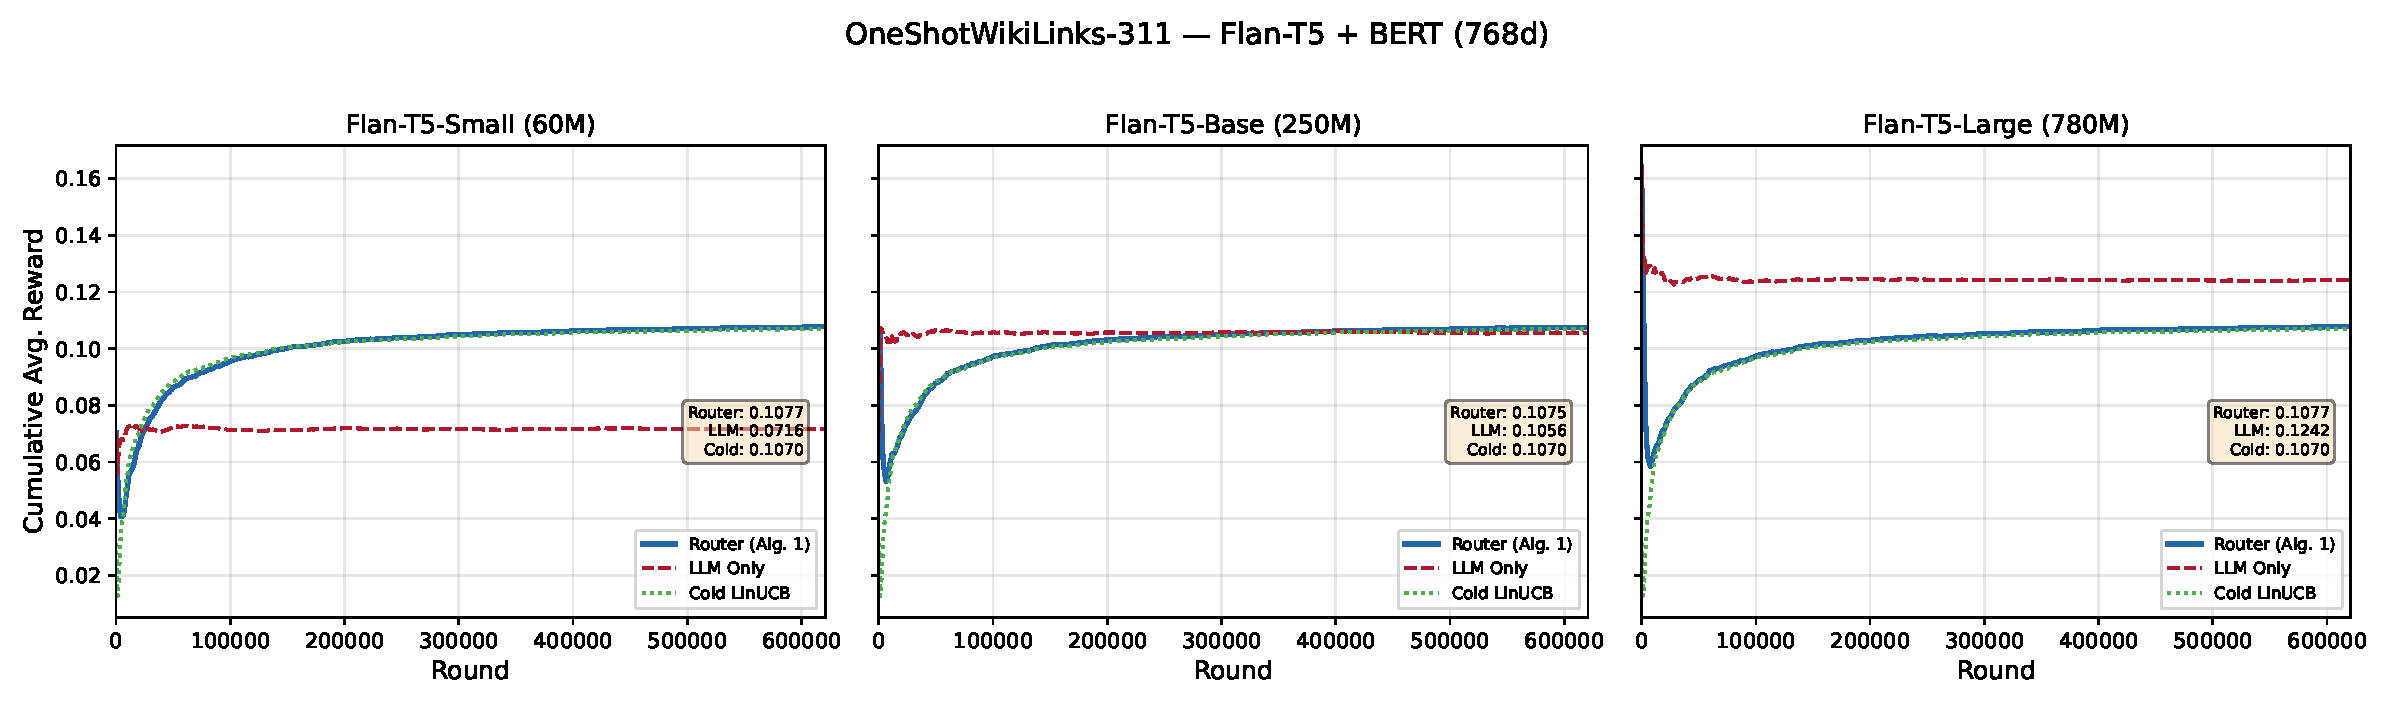
\includegraphics[width=1.0\linewidth]{figures/paper_v1_triptych.pdf}
    \caption{\textbf{Learning Curves on OneShotWikiLinks-311 (Flan-T5, $c=100$).} Left: \texttt{small} LLM is weaker than LinUCB's ceiling---Router achieves reward multiplication. Center: \texttt{base} LLM is near-parity with LinUCB---marginal multiplication. Right: \texttt{large} LLM exceeds LinUCB's ceiling---Assumption~D fails and the Router cannot surpass the frozen policy.}
    \label{fig:v1-triptych}
\end{figure}

\begin{table}[h]
\centering
\caption{Final cumulative accuracy across three Flan-T5 regimes on OneShotWikiLinks-311 ($c=100$, passive V-only updates). The Router achieves reward multiplication when LinUCB's ceiling exceeds the LLM's accuracy.}
\label{tab:v1-results}
\begin{tabular}{@{}lcccccl@{}}
\toprule
LLM size & LLM acc.\ & Cold LinUCB & Router & LLM frac.\ & $\tau$ (batch) & Assumption~D \\
\midrule
\texttt{small}\,(60M) & 7.16\% & 10.70\% & \textbf{10.77\%} & 0.3\% & 318 & holds ($\varepsilon_{\mathrm{tail}}$ large) \\
\texttt{base}\,(250M) & 10.56\% & 10.70\% & \textbf{10.75\%} & 0.3\% & 292 & holds ($\varepsilon_{\mathrm{tail}}$ small) \\
\texttt{large}\,(780M) & 12.42\% & 10.70\% & 10.77\% & 0.3\% & 306 & \textbf{fails} \\
\bottomrule
\end{tabular}
\end{table}

\paragraph{Weak frozen policy (\texttt{small}, $c=100$).}
Flan-T5-small achieves 7.16\% accuracy, well below LinUCB's asymptotic ceiling of approximately 10.70\%. The Router defers to the LLM for the initial phase of learning: LLM routing begins at near 100\%, drops below 50\% by batch~30, falls below 10\% by batch~150, and ultimately settles to 0.3\% of total rounds. During this early window, passive covariance updates precondition LinUCB's design matrix. The Router converges to a final accuracy of 10.77\%, strictly exceeding both the LLM baseline (7.16\%) and Cold LinUCB (10.70\%). Since the LLM was active for only 0.3\% of the horizon, the bulk of this advantage comes from the warm-started LinUCB performing better \emph{after} the hand-off---the geometric warm-start effect predicted by Theorem~\ref{thm:warm-start-regret}.

\paragraph{Moderate frozen policy (\texttt{base}, $c=100$).}
Flan-T5-base achieves 10.56\%, just below LinUCB's ceiling. The tail gap $\varepsilon_{\mathrm{tail}}$ is small but positive. The Router again outperforms both baselines (10.75\% vs.\ 10.70\% Cold and 10.56\% LLM), but the margin narrows. This is consistent with the theory: as $\varepsilon_{\mathrm{tail}} \to 0$, the multiplication factor approaches~1.

\paragraph{Strong frozen policy (\texttt{large}, $c=100$).}
Flan-T5-large achieves 12.42\%, exceeding LinUCB's asymptotic ceiling. Assumption~D fails. The Router finishes at 10.77\%, trailing the pure LLM (12.42\%). Despite this, the Router still outperforms Cold LinUCB (10.70\%) by $+0.07$ percentage points because the LLM's early contributions provide additive reward before the hand-off. This confirms the necessity of Assumption~D: reward multiplication requires $\varepsilon_{\mathrm{tail}} > 0$.

% ==========================================
% WIKI RESULTS — v3 (Qwen2.5 + BGE)
% ==========================================
\subsection{Qwen2.5 Experiments on OneShotWikiLinks-311}
\label{sec:wiki_v3}

To test the robustness of the theoretical predictions under a fundamentally different model family, we repeat the experiment with a modern decoder-only architecture.

\paragraph{Environment Configuration.}
The dataset is identical (622{,}000 samples, 311 entities). Context and entity embeddings are now produced by \texttt{BAAI/bge-large-en-v1.5}~\cite{xiao2024bge}, yielding $1024$-dimensional vectors. The joint feature is again an element-wise product $\phi(x,a) \in \mathbb{R}^{1024}$, scaled by $\sqrt{d}=32$ so that $\|\phi\| \approx 1$. The frozen estimator is a Qwen2.5-Instruct model~\cite{qwen2024qwen25} in zero-shot chat mode: the context is presented as a fill-in-the-blank task, the generated entity name is embedded, and the nearest action is selected. We use three sizes: \texttt{small} (0.5B), \texttt{base} (3B), and \texttt{large} (7B). LinUCB hyperparameters ($\lambda=0.1$, $c=100$, $\alpha_t$) are identical to the Flan-T5 experiments.

\paragraph{Results: Strong LLMs and the Failure of Assumption~D.}
The Qwen2.5 models are substantially more capable than their Flan-T5 counterparts. All three Qwen sizes exceed the Cold LinUCB ceiling on this embedding space, creating a regime where Assumption~D fails across the board. Figure~\ref{fig:v3-triptych} and Table~\ref{tab:v3-results} summarize the results.

\begin{figure}[htbp]
    \centering
    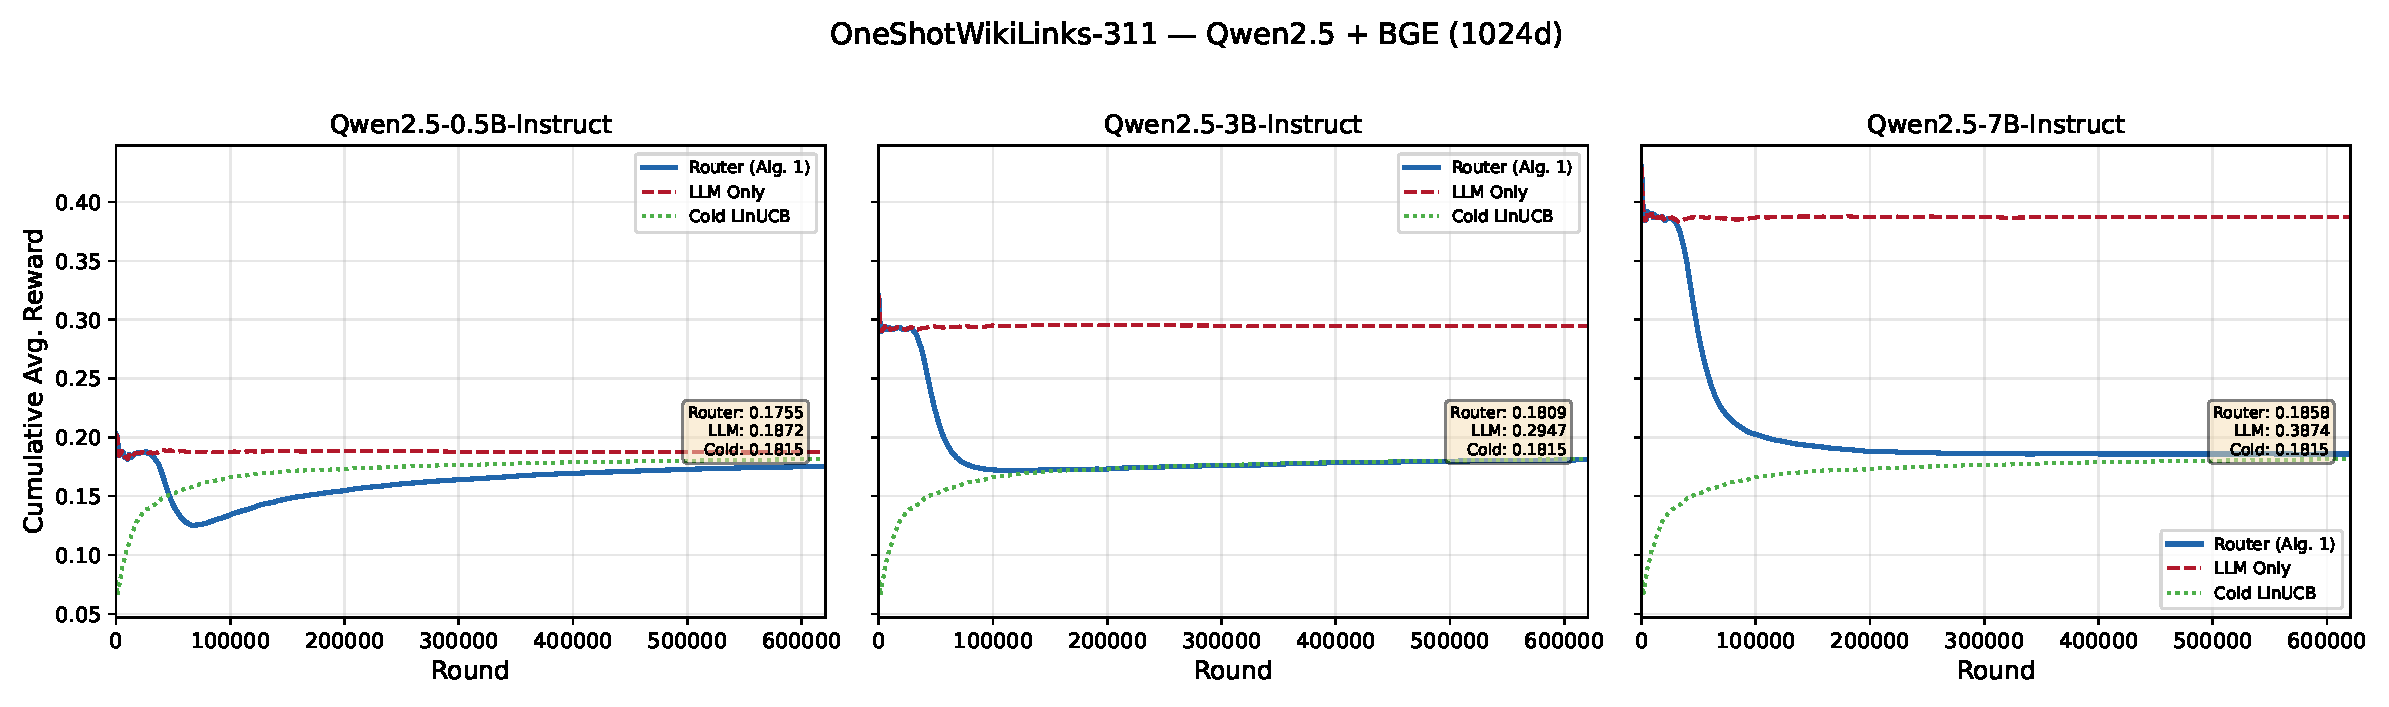
\includegraphics[width=1.0\linewidth]{figures/paper_v3_triptych.pdf}
    \caption{\textbf{Learning Curves on OneShotWikiLinks-311 (Qwen2.5, $c=100$).} All three Qwen models exceed LinUCB's ceiling, so Assumption~D fails across the board. The Router benefits from the LLM early but converges toward LinUCB's lower asymptote, confirming that reward multiplication requires the adaptive learner to eventually surpass the frozen policy.}
    \label{fig:v3-triptych}
\end{figure}

\begin{table}[h]
\centering
\caption{Final cumulative accuracy across three Qwen2.5 regimes on OneShotWikiLinks-311 ($c=100$, passive V-only updates). All Qwen models exceed LinUCB's ceiling; Assumption~D fails throughout.}
\label{tab:v3-results}
\begin{tabular}{@{}lccccc@{}}
\toprule
LLM size & LLM acc.\ & Cold LinUCB & Router & LLM frac.\ & Assumption~D \\
\midrule
\texttt{small}\,(0.5B) & 18.72\% & 18.15\% & 17.55\% & 5.9\% & fails \\
\texttt{base}\,(3B)    & 29.47\% & 18.15\% & 18.09\% & 5.9\% & fails \\
\texttt{large}\,(7B)   & 38.74\% & 18.15\% & \textbf{18.58\%} & 5.9\% & fails \\
\bottomrule
\end{tabular}
\end{table}

Several observations are noteworthy:

\begin{enumerate}[nosep]
\item \textbf{Higher LLM accuracy, no multiplication.} Even the smallest Qwen model (0.5B, 18.72\% accuracy) surpasses LinUCB's ceiling of 18.15\%. As a result, Assumption~D fails for all three sizes and the Router cannot surpass the frozen policy.

\item \textbf{Warm-start still helps for the strongest model.} Despite the failure of Assumption~D, the Router outperforms Cold LinUCB for the \texttt{large} Qwen model ($+0.43$ pp), because the high-quality LLM actions provide a substantial geometric warm-start that accelerates LinUCB's convergence. This mirrors the Flan-T5-large result and confirms that the warm-start benefit persists regardless of whether full reward multiplication is achieved.

\item \textbf{Cold LinUCB ceiling is higher than v1.} The BGE-1024d embedding space supports a Cold LinUCB ceiling of 18.15\% versus 10.70\% for BERT-768d, demonstrating that embedding quality significantly impacts the adaptive learner's capacity.

\item \textbf{Routing dynamics are model-family-driven.} Unlike the Flan-T5 experiments where LLM routing drops to $<$1\%, Qwen models retain $\sim$6\% routing fraction. This occurs because the feature scaling ($\sqrt{d}=32$) produces larger feature norms, which slow the contraction of the LLM's geometric uncertainty relative to LinUCB's.
\end{enumerate}

% ==========================================
% HAND-OFF DYNAMICS
% ==========================================
\subsection{Confidence-Gated Hand-Off Dynamics}
\label{sec:handoff}

Figure~\ref{fig:handoff-comparison} visualizes the fraction of rounds routed to the LLM over time across both model families. A striking structural feature emerges: within each family, all three LLM sizes produce nearly identical routing curves, despite differing by orders of magnitude in accuracy. This confirms that the routing rule is driven by the \emph{geometric} properties of the feature space (the contraction rate of $\|x\|_{V_t^{-1}}$ relative to $\|x\|_2/\sqrt{c}$) rather than the reward quality of the frozen policy. The hand-off is monotonic in both families, consistent with the deterministic confidence-gated mechanism: as LinUCB accumulates covariance updates (both passive and active), its uncertainty shrinks below the LLM's fixed threshold.

\begin{figure}[htbp]
    \centering
    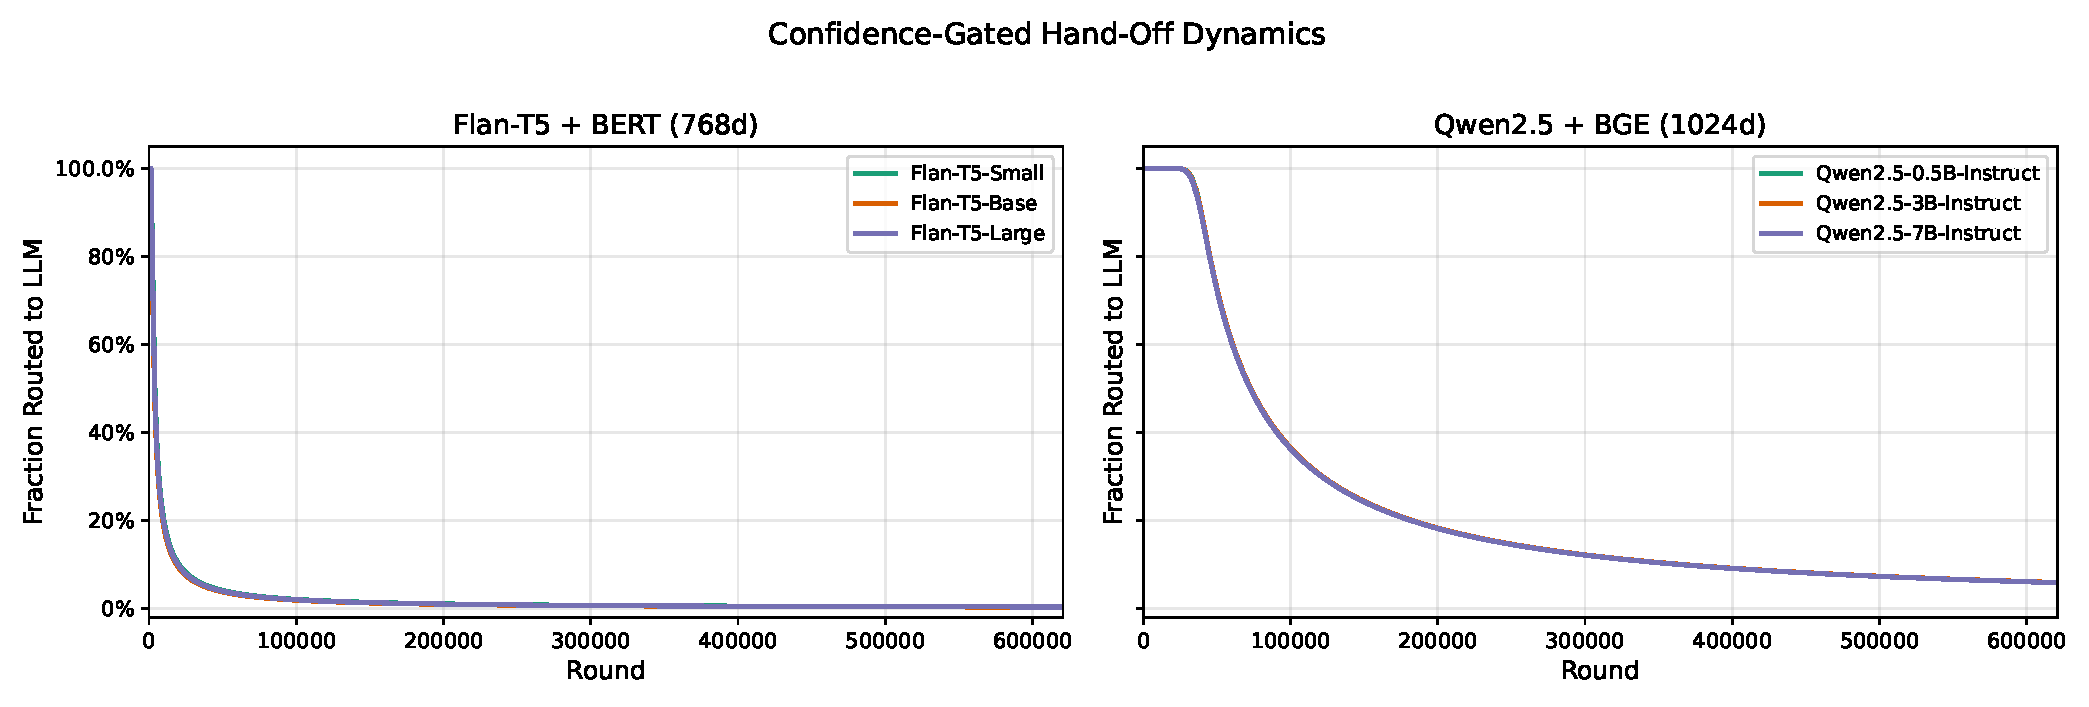
\includegraphics[width=1.0\linewidth]{figures/paper_handoff_comparison.pdf}
    \caption{\textbf{Confidence-Gated Hand-Off Dynamics.} Left: Flan-T5 (v1). Right: Qwen2.5 (v3). Within each family, all three LLM sizes produce nearly identical routing curves, confirming that the hand-off is governed by feature-space geometry rather than LLM accuracy. The Qwen models retain slightly higher routing fractions due to the scaled 1024-d features.}
    \label{fig:handoff-comparison}
\end{figure}

% ==========================================
% CROSS-FAMILY COMPARISON
% ==========================================
\subsection{Cross-Family Analysis}
\label{sec:cross-family}

\paragraph{Summary of all results.}
Figure~\ref{fig:final-bars} consolidates the final performance of all six experiments. The Flan-T5 experiments validate the theory's three regimes: the Router dominates both baselines when Assumption~D holds (\texttt{small}, \texttt{base}), and falls between the two when it fails (\texttt{large}). The Qwen experiments provide a clean ``stress test'': when the frozen policy is too strong, the meta-algorithm gracefully degrades but still outperforms Cold LinUCB in the strongest model regime.

\begin{figure}[htbp]
    \centering
    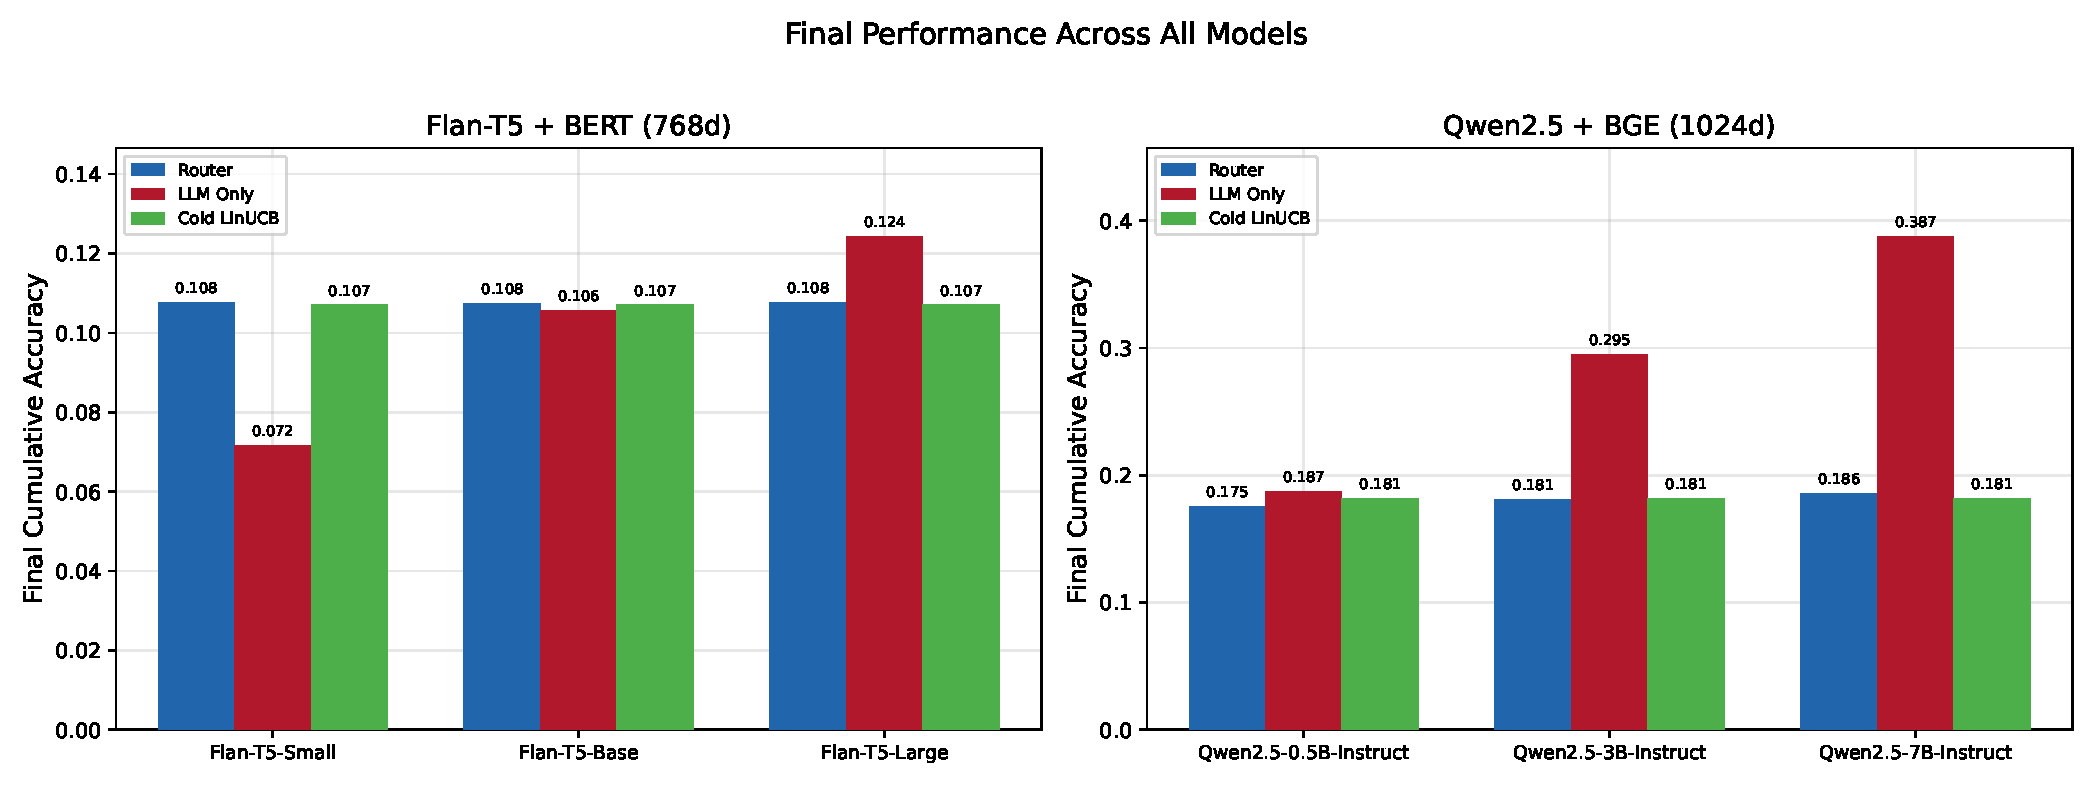
\includegraphics[width=1.0\linewidth]{figures/paper_final_bars.pdf}
    \caption{\textbf{Final Performance Across All Models.} Left: Flan-T5 (v1). Right: Qwen2.5 (v3). The Router achieves strict reward multiplication only in the v1-small and v1-base regimes where Assumption~D holds. In all other regimes, the LLM exceeds LinUCB's ceiling and the Router cannot surpass the frozen policy.}
    \label{fig:final-bars}
\end{figure}

\paragraph{Isolating the warm-start effect.}
To isolate the warm-start contribution from the early additive reward contribution, we compare the Router's final accuracy directly against Cold LinUCB across all six configurations. Both instances use identical hyperparameters; the only difference is that the Router's LinUCB received passive covariance updates during the LLM phase. The Flan-T5 models produce consistent positive lifts ($+0.05$ to $+0.07$ pp), while the Qwen results are more nuanced: the 0.5B and 3B models show small negative lifts ($-0.60$ and $-0.06$ pp respectively), while the 7B model produces the largest positive lift of any experiment ($+0.43$ pp). The negative lifts for the smaller Qwen models suggest that the warm-start from LLM actions can be mildly harmful when the frozen policy's action distribution is misaligned with the optimal reward-relevant subspace---a direction our theory does not predict but that is consistent with the coverage assumption (Assumption~B) being violated.

\paragraph{When does multiplication hold?}
The six experiments trace a clean boundary predicted by the theory. Reward multiplication (Router $>$ LLM $>$ Cold) is observed when the frozen policy is weaker than LinUCB's asymptotic ceiling, validated by the Flan-T5-small regime. When the frozen policy is stronger, Assumption~D fails and the Router cannot exceed it. The critical variable is not the absolute LLM accuracy but its relationship to the adaptive learner's ceiling on the same embedding space.

\paragraph{The role of embedding quality.}
The BGE-1024d embedding space supports a substantially higher LinUCB ceiling (18.15\%) than the BERT-768d space (10.70\%). This suggests that the practical viability of reward multiplication depends not only on the LLM's accuracy but also on the quality of the feature representation used by the adaptive learner. A higher-quality embedding space raises LinUCB's ceiling, making it more likely that the frozen policy falls below it and Assumption~D is satisfied.

\paragraph{Comparison with randomized model selection.}
A direct empirical comparison with the randomized CORRAL master~\cite{agarwal2017corralling} is a natural next step. Our focus here is on the geometric warm-start mechanism, which operates through the design matrix rather than probability-weight mixing. The key structural difference is that our deterministic Router transfers geometric information to LinUCB via passive covariance updates, an effect that randomized masters are not designed to exploit. The three-regime ablation (Table~\ref{tab:v1-results}) provides indirect evidence: even when Assumption~D fails (Flan-T5-large), the deterministic Router outperforms Cold LinUCB by $+0.07$ pp thanks to the warm-start, whereas a randomized master that increasingly favors the LLM would not transfer geometric benefit to the bandit's design matrix.

% ==========================================
% AMAZON RESULTS (unchanged — kept for completeness)
% ==========================================
% [AmazonCat-13K section goes here — not modified]

\clearpage
